%%%%%%%%%%%%%%%%%%%%%%%%%%%%%%%%%%%%%
%%%%%%%%%%%%%%%%%%%%%%%%%%%%%%%%%%%%%
\documentclass{article}

\usepackage[preprint,nonatbib]{neurips_2024}

\usepackage[utf8]{inputenc} % allow utf-8 input
\usepackage[T1]{fontenc}    % use 8-bit T1 fonts
\usepackage{hyperref}       % hyperlinks
\usepackage{url}            % simple URL typesetting
\usepackage{booktabs}       % professional-quality tables
\usepackage{amsfonts}       % blackboard math symbols
\usepackage{nicefrac}       % compact symbols for 1/2, etc.
\usepackage{microtype}      % microtypography
\usepackage{xcolor}         % colors
\usepackage{amsmath}
\usepackage{pgfplots}
\usepackage{caption}  % To add a caption
\usepackage{tcolorbox} % For creating colored or framed boxes
\usepackage{subcaption}
\usepackage[noabbrev,capitalise]{cleveref}


\pgfplotsset{compat=1.18}

%%%%%%%%%%%%%%%%%%%%%%%%%%%%%%%%%%%%%
\title{Assignment \#4\\
  \vspace{2mm}
  \small{Elements of Machine Learning}
  \\
  \vspace{2mm}
  \small{Saarland University -- Winter Semester 2024/25}
}

\author{%
\textbf{Rabin Adhikari} \\
  7072310 \\
  \texttt{raad00002@stud.uni-saarland.de} \\
  \and
  \textbf{Dhimitrios Duka} \\
 7059153 \\
  \texttt{dhdu00001@stud.uni-saarland.de} \\
}

%%%%%%%%%%%%%%%%%%%%%%%%%%%%%%%%%%%%%
\begin{document}
\maketitle

%%%%%%%%%%%%%%%%%%%%%%%%%%%%%%%%%%%%%
\setcounter{section}{1}
\section{Problem 2 (Hierarchical clustering and dissimilarity)}
\subsection{To perform k-means clustering, k-medoids, or agglomerative clustering, is it necessary to know the coordinates of the elements being clustered, or is it sufficient to have only their dissimilarity matrix? Explain your answer in detail.}
Out of the three mentioned clustering methods, only $k$-means requires the coordinates of the elements being clustered. This is because, at each iteration of the algorithm, $k$-means needs to find the mean of all data points in a given cluster $C_i$. In contrast, both $k$-medoids and agglomerative clustering can work with just the dissimilarity matrix, as they don't create new points, such as the mean of the cluster, or perform coordinate-based calculations. $k$-medoids select actual data points as cluster centers and use only pairwise dissimilarities for cluster assignments, while agglomerative clustering builds a hierarchy by progressively merging clusters based solely on dissimilarities between existing points. For $k$-medoids and agglomerative clustering, coordinates are more of a proxy for calculating the dissimilarity scores. Therefore, having direct access to the dissimilarity scores renders the coordinates useless.

\subsection{The hierarchical clustering algorithm has already identified one cluster, and the dissimilarity matrix below represents the pairwise dissimilarities among the elements...}
\subsubsection{Complete linkage}
First, we will start by finding the two most similar clusters. From the given dissimilarity matrix, we can conclude that the two clusters with the minimum dissimilarity score are cluster $C$ and $D$. These two clusters would merge and form a new cluster $[C, D]$. Additionally, while updating the similarity matrix, we will choose the maximum dissimilarity between clusters as the new value for the dissimilarity. The resulting similarity matrix is given in the table below:

\begin{center}
    \begin{tabular}{c|ccc}
          & \{A,B\} & \{C,D\} & E \\
    \hline
    \{A,B\} & 0     & 1.8   & 2.3 \\
    \{C,D\} & 1.8   & 0     & 1.7 \\
    E       & 2.3   & 1.7   & 0   \\
    \end{tabular}
\end{center}

\subsubsection{Single linkage}
For the single linkage method, we will follow a similar approach to the Complete linkage method. First, we will merge the two most similar clusters, and then we will update the similarity matrix. As in the previous exercise, we will merge clusters $C$ and $D$. However, while updating the similarity matrix, we will choose the minimum distance between clusters instead of the maximum. The resulting similarity matrix is given in the table below:

\begin{center}
    \begin{tabular}{c|ccc}
          & \{A,B\} & \{C,D\} & E \\
    \hline
    \{A,B\} & 0     & 1.2   & 2.3 \\
    \{C,D\} & 1.2   & 0     & 1.4 \\
    E       & 2.3   & 1.4   & 0   \\
    \end{tabular}
\end{center}

\subsubsection{}
The final dendogram is shown in Figure\ref{fig:dendogram}. First, clusters $\{A\}$ and $\{B\}$ are merged. Next, clusters $\{C\}$ and $\{D\}$. Next clusters $\{A, B\}$ and $\{C, D\}$ are merged. And finally, clusters $\{A, B, C, D\}$ and $\{E\}$ are merged.
\begin{figure}[h!]
    \centering
    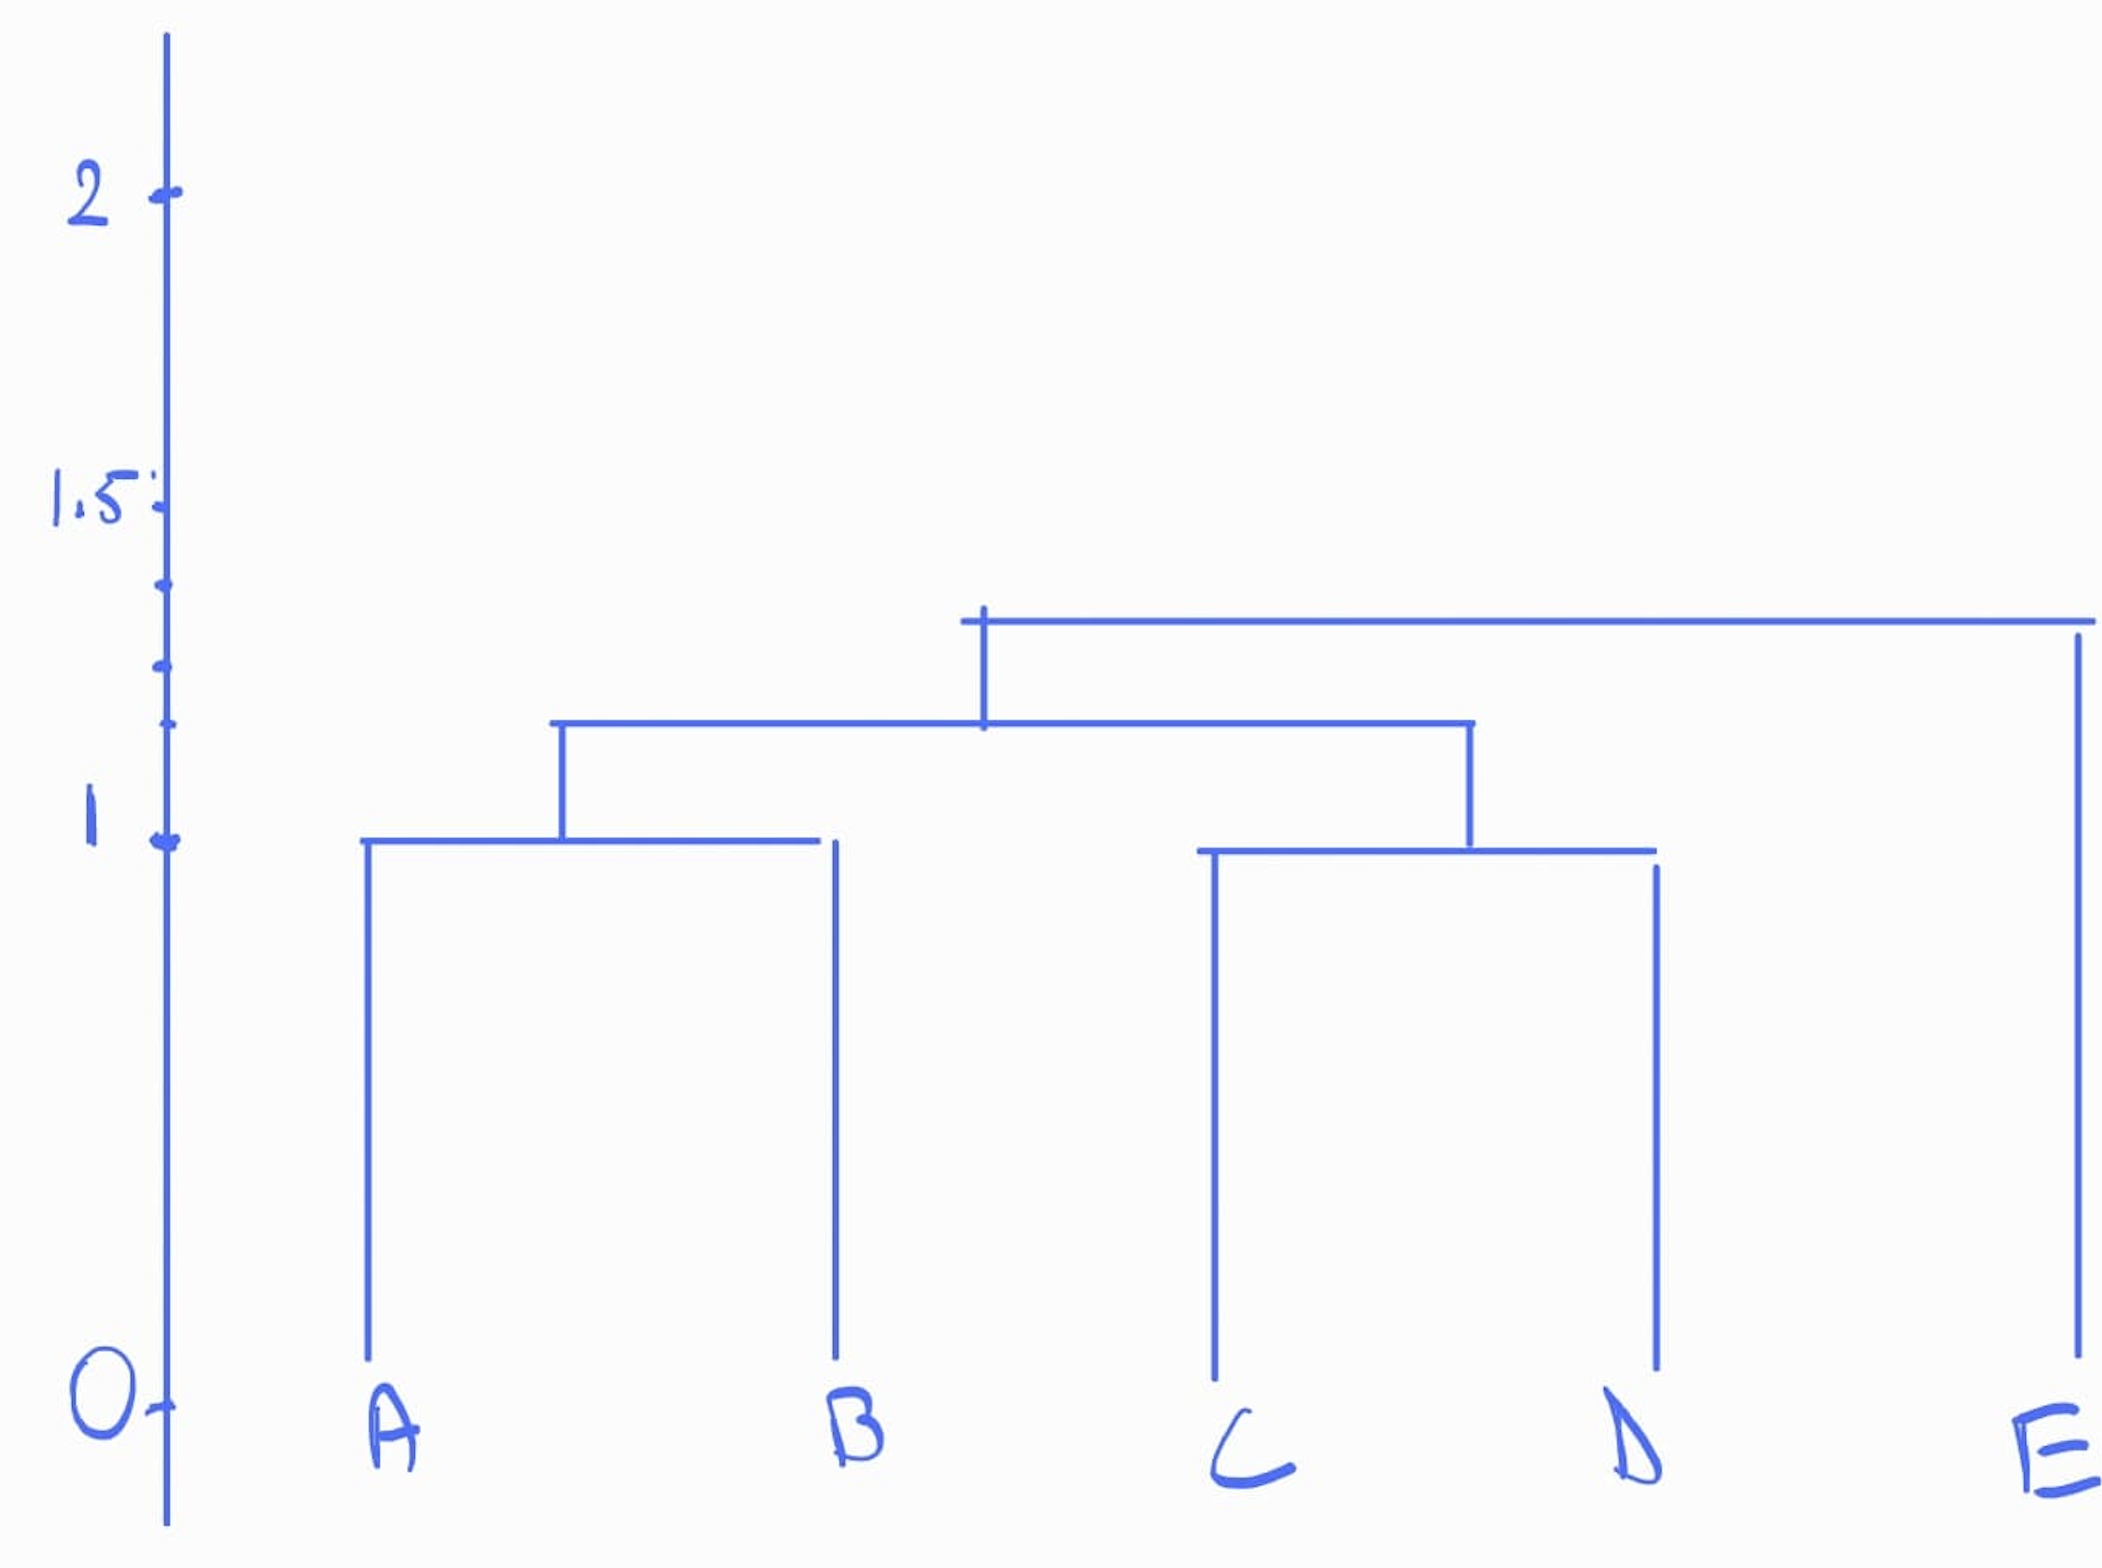
\includegraphics[width=0.5\textwidth]{dendogram.png}
    \caption{Resulting dendogram from the provided steps.}
    \label{fig:dendogram}
\end{figure}

%%%%%%%%%%%%%%%%%%%%%%%%%%%%%%%%%%%%%
\clearpage

%%%%%%%%%%%%%%%%%%%%%%%%%%%%%%%%%%%%%
% \bibliographystyle{unsrt}
% \bibliography{references}

%%%%%%%%%%%%%%%%%%%%%%%%%%%%%%%%%%%%%
%%%%%%%%%%%%%%%%%%%%%%%%%%%%%%%%%%%%%
\end{document}

%%%%%%%%%%%%%%%%%%%%%%%%%%%%%%%%%%%%%
%%%%%%%%%%%%%%%%%%%%%%%%%%%%%%%%%%%%%